\documentclass{oblivoir}
\usepackage{graphicx}
\usepackage{ikps,ansform}
  \newcounter{problem}[section]
    \newenvironment{problem}{\noindent\refstepcounter{problem}\textbf{\large\theproblem.} }{}\documentclass{article}
\usepackage[utf8x]{inputenc}


\begin{document}
그림과 같이 물체가 높이 $h$인 곳에서 가만히 출발하여 마찰이 없는 면의 따라 높이 $2h$인 곳에 도달한다. 물체는 수평면 구간 A와 B를 지나는 도중에 각각 운동 방향으로 크기가 같은 힘 F를 같은 시간 동안 받는다. 높이 $2h$인 곳에 도달하였을 때 물체의 속력은 0이다. 
\begin{figure}[h!]
    \centering
    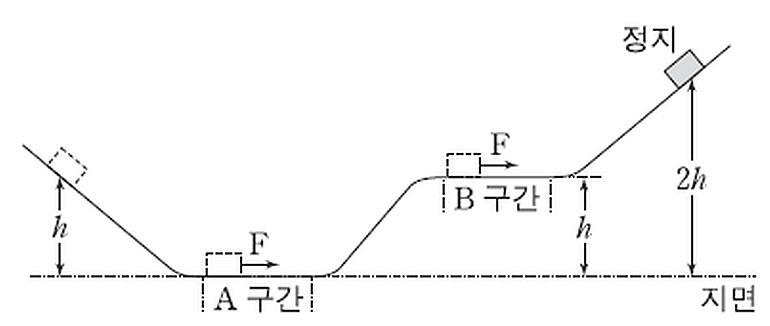
\includegraphics[scale=0.5]{170920.png}}
\end{figure}
        \par
A에서 F가 물체에 한 일을 $W_A$, B에서 F가 물체에 한 일을 $W_B$라 할 때, $\dfrac{W_B}{W_A}$는? (단, 물체의 크기와 공기 저항은 무시한다.)
\ansone{\dfrac{2}{3}}{\dfrac{7}{9}}{\dfrac{8}{9}}{1}{\dfrac{10}{9}}
\section{풀이}
물체가 A구간에 진입하기전 바닥에서의 속도를 $v$라 합시다.
물체가 B구간을 지난후 $h$만큼 올라갔을때 속력이 0이 되었으므로 A구간전의 물체의 높이를 $h$만큼 올린것과 같습니다. 다시 말해서 B구간을 지난 직후의 물체의 속력은 $v$입니다. A구간과 B구간의 공통점은 충격량이 같다는건데 이는 구간을 지난후의 속도 상승량이 같습니다. 이 속도 상승량을 $\Delta v$라고 합시다. 그러면 A구간을 지난 직후의 물체의 속력은 $v+\Delta v$이고 B구간을 지나기 직전의 속력은 $v-\Delta v$입니다. 
\par
물체의 질량을 $m$이라 하면 
\par
$W_A=\dfrac{1}{2}m((v+\Delta v)^2-v^2)$ 
\par
$W_B = \dfrac{1}{2}m(v^2-(v-\Delta v)^2)$
\par
$W_A + W_B = \dfrac{1}{2}m v^2$\par 이를 정리하면 $\Delta v =\dfrac{1}{4}v$가 나옵니다. 이를 이용해서 $\dfrac{W_B}{W_A}$를 계산하는데 어짜피 알아서 소거되기 때문에 $v^2$의 계수만 계산을 하면됩니다. \par $\dfrac{1-\left(\dfrac{3}{4}\right)^2}{\left(\dfrac{5}{4}\right)^2-1}$ 정리하면 2번이 답입니다.
\par \par \par \par
혹시 속력이 아닌 운동량으로 분석했을 경우는 A구간 진입 직전 운동량을 $p$, 구간을 지났을때의 충격량을 $\Delta p$라고 하면\par $W_A=\dfrac{((p+\Delta p)^2-p^2)}{2m}$ \par $W_B = \dfrac{(p^2-(p-\Delta p)^2)}{2m}$ \par
$W_A + W_B = \dfrac{p^2}{2m}$으로 식을 놓을 수 있습니다. 계산 방향은 같습니다. 
\newpage
\section{역학적 에너지 보존 동치식}
보지말고 직접한번 해봅시다.
\begin{figure}[h!]
    \centering
    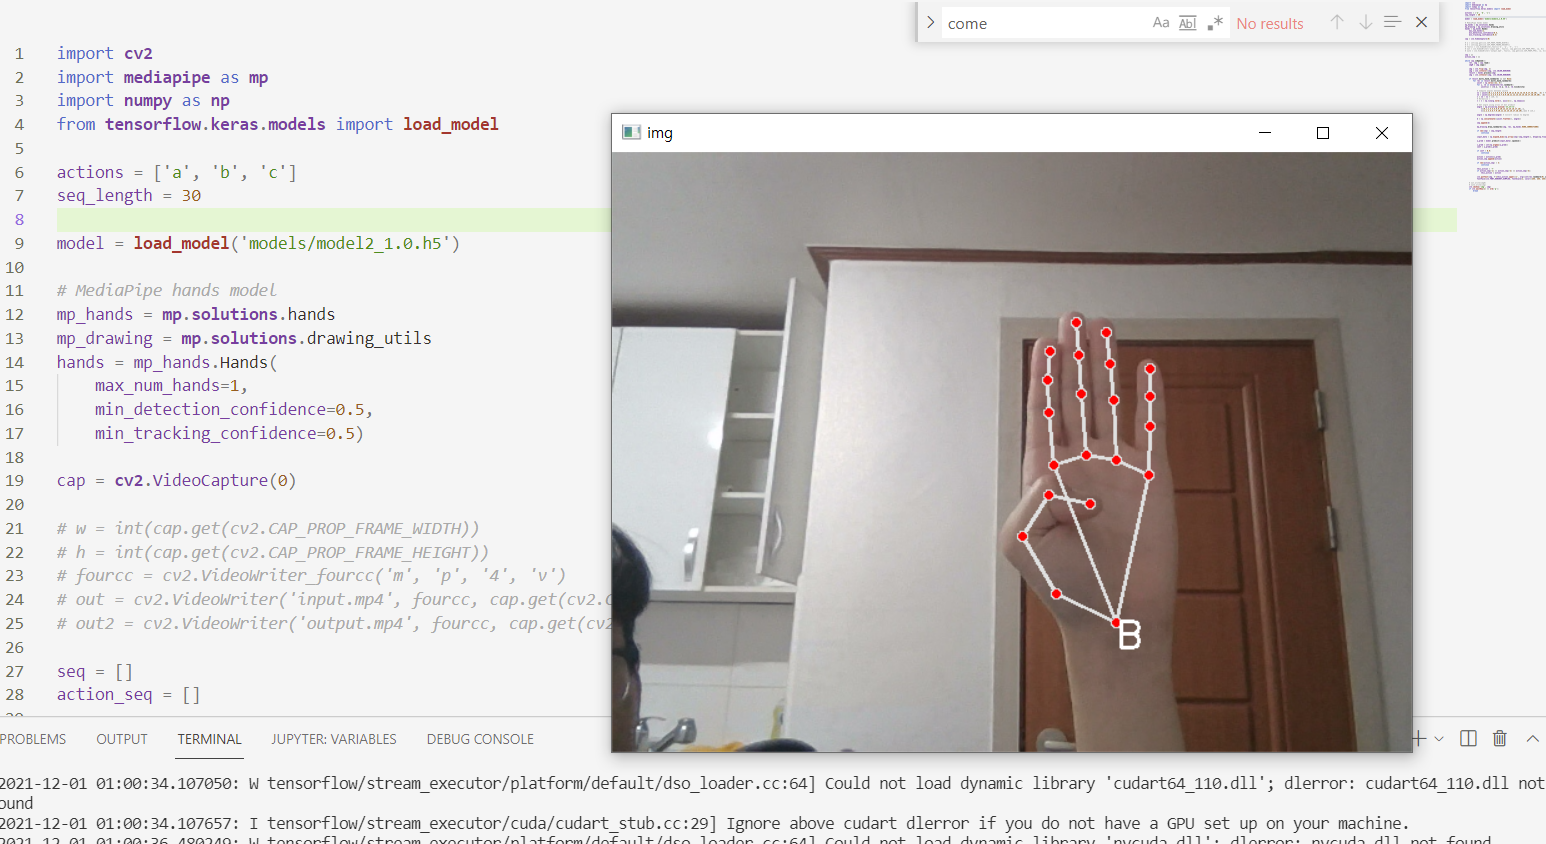
\includegraphics[scale =0.5]{B.PNG}
    \label{fig:my_label}
\end{figure}
물체질량을 $m$이라 하고 구간동안 충격량을 $I$, 속도 변화량을 $\Delta v$라 합시다.
\begin{enumerate}
    \item 처음정지구간: $mgh$
    \item A구간 진입 전: 1과 같다. $mgh = \dfrac{1}{2}mv^2$
    \item  A구간 진입 후: $mgh + W_A  =\dfrac{1}{2}mv^2 + W_A = \dfrac{1}{2}m(v+\Delta v)^2 = \dfrac{(mv + I)^2}{2m}$ \begin{justbox}
    절대로 운동량을 운동에너지 식으로 바꿀때 단순 덧셈으로
    $\dfrac{(mv)^2}{2m}+\dfrac{I^2}{2m}$으로 하지않도록 주의 
    \end{justbox}
    \item  B구간 진입 전: 3과 같다.\par
    $mgh + W_A  =\dfrac{1}{2}mv^2 + W_A = \dfrac{1}{2}m(v+\Delta v)^2 = \dfrac{(mv + I)^2}{2m} = \dfrac{1}{2}m(v-\Delta v)^2 + mgh = \dfrac{1}{2}m(v-\Delta v)^2 + \dfrac{1}{2}mv^2= \dfrac{(mv - I)^2}{2m} +mgh$
    \item B구간 진입 후:   $mgh + W_A + W_B = \dfrac{1}{2}mv^2 + W_A + W_B = \dfrac{1}{2}m(v+\Delta v)^2 + W_B = \dfrac{(mv + I)^2}{2m} + W_B = \dfrac{1}{2}m(v-\Delta v)^2 + mgh + W_B = \dfrac{1}{2}m(v-\Delta v)^2 + \dfrac{1}{2}mv^2 + W_B = \dfrac{(mv - I)^2}{2m} + mgh + W_B = \dfrac{1}{2}mv^2 + mgh $
    \item $2h$도달: 5와 같다. $mg(2h)$
\end{enumerate}
\end{document}
